\chapter{Integration avec l'outil de facturation}
\label{chap:integration-facturation}

\section{Objectif du sprint 7}

Le sprint 7 correspondait au Backlog Item 71 et aux taches 83 et 84. Son objectif etait d'integrer les donnees extraites avec un outil de facturation accessible via Power Apps. La solution devait permettre une synchronisation bidirectionnelle entre Postgres, Microsoft Dataverse et l'interface utilisateur.

\begin{figure}[H]
\center
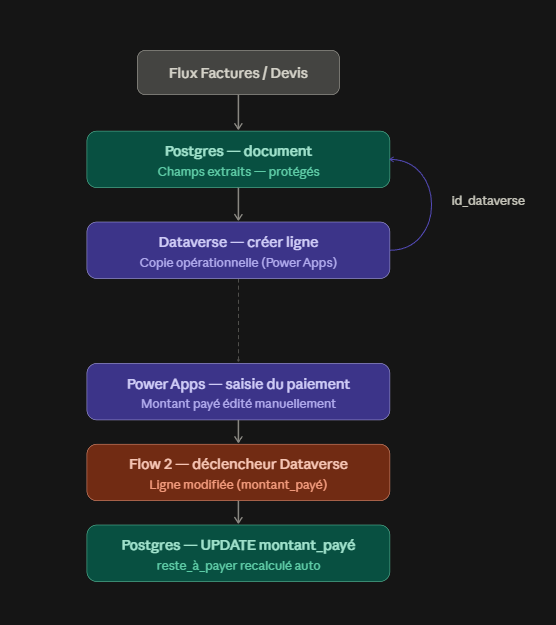
\includegraphics[width=0.9\textwidth]{images/architecture.png}
\caption[Architecture d'integration]{Architecture globale de synchronisation entre Postgres, Dataverse et Power Apps.}
\label{fig:architecture-integration}
\end{figure}

\section{Synchronisation Postgres vers Dataverse}

Le premier flux Power Automate cree une copie operationnelle dans Dataverse a chaque nouveau document insere dans Postgres. Cette copie contient les champs necessaires a l'utilisation dans Power Apps. Le lien entre les deux environnements est conserve grace au champ \texttt{id\_dataverse}.

\begin{figure}[H]
\center
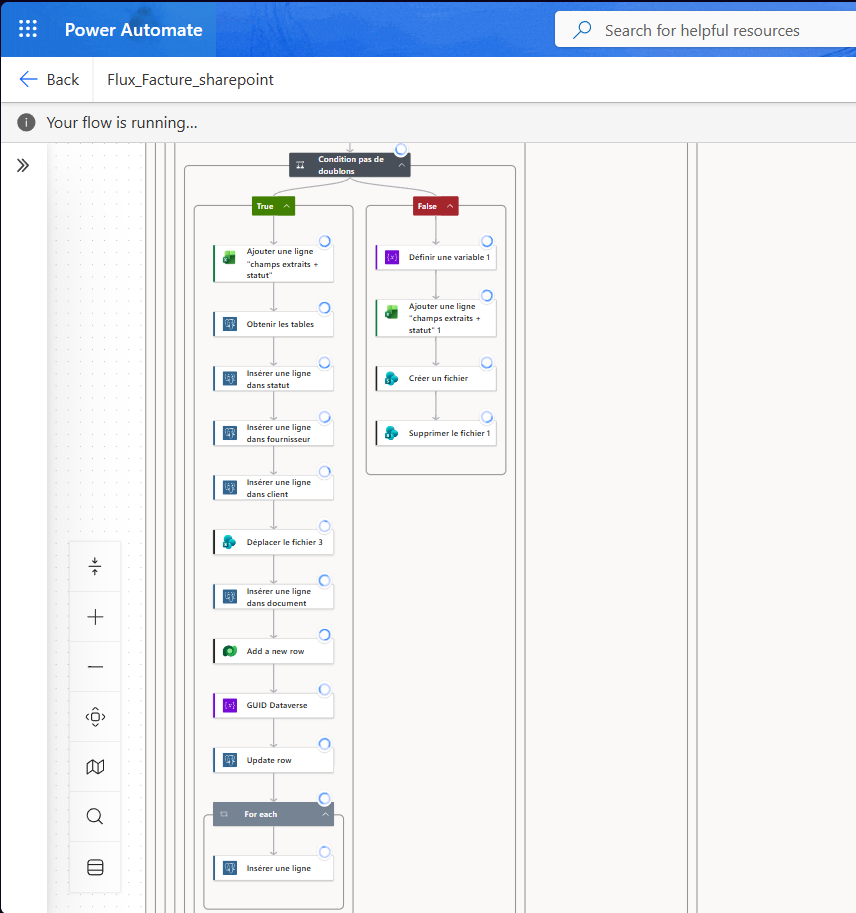
\includegraphics[width=0.85\textwidth]{images/flow1.png}
\caption[Flux de creation Dataverse]{Flux Power Automate responsable de la creation d'une entree Dataverse depuis Postgres.}
\label{fig:flow1}
\end{figure}

La modelisation Dataverse a ete testee avec deux tables representant les documents et leurs attributs utiles pour l'outil de facturation.

\begin{figure}[H]
\center
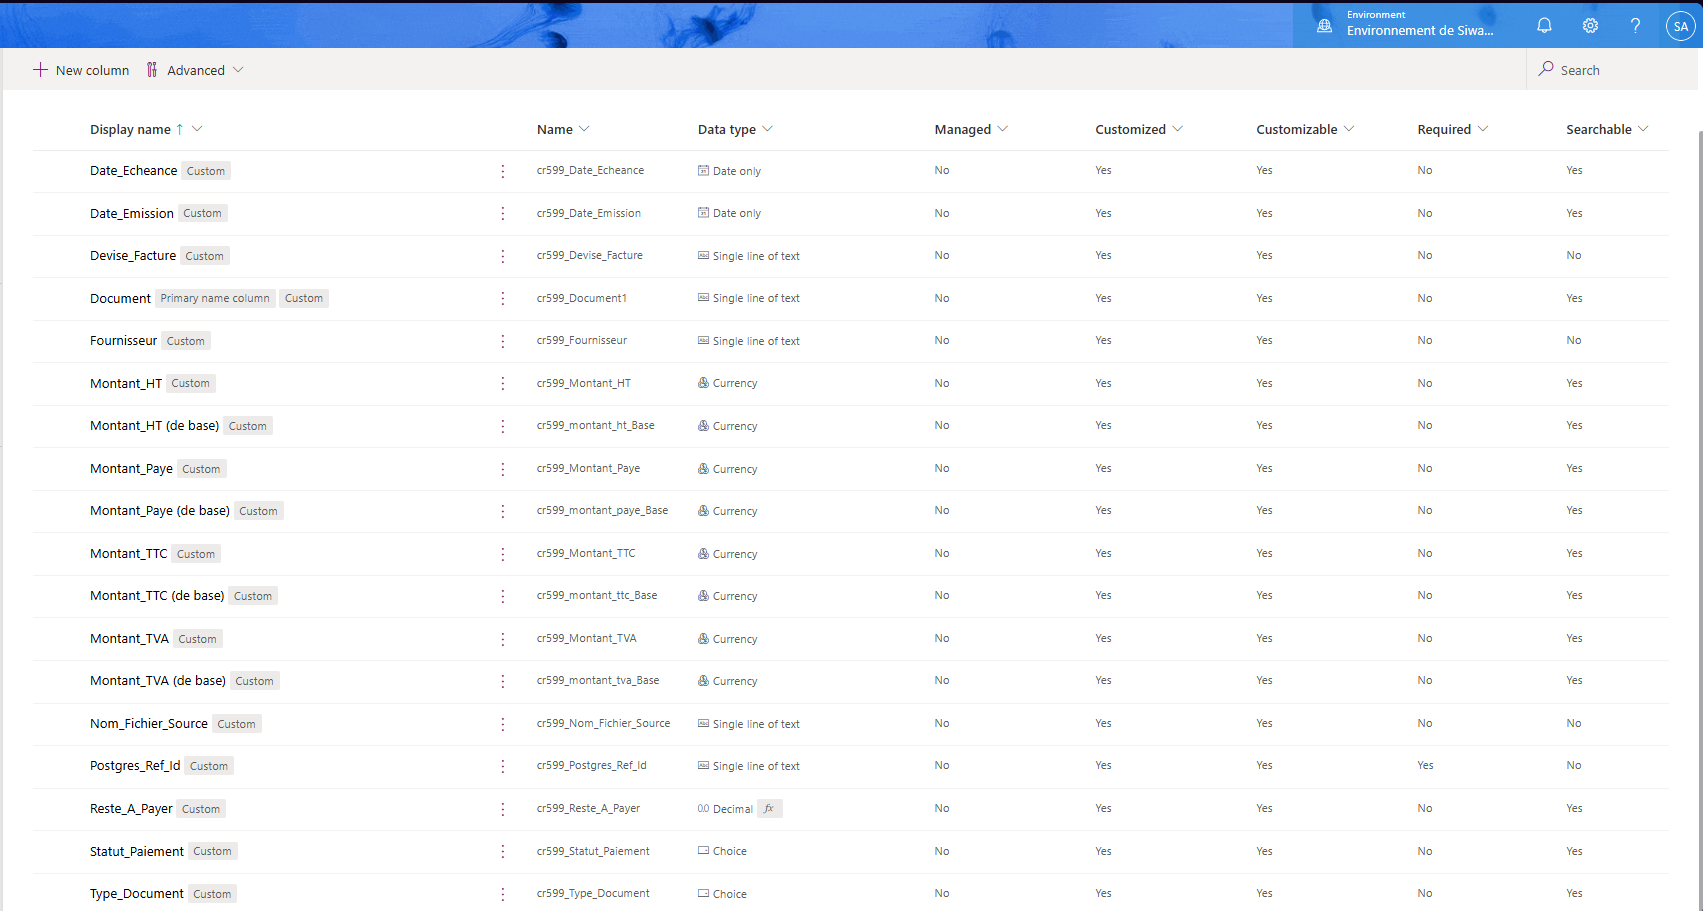
\includegraphics[width=0.85\textwidth]{images/table_Document_Dataverse.png}
\caption[Table Document Dataverse]{Table Dataverse utilisee pour representer les informations principales d'un document.}
\label{fig:table-document-dataverse}
\end{figure}

\begin{figure}[H]
\center
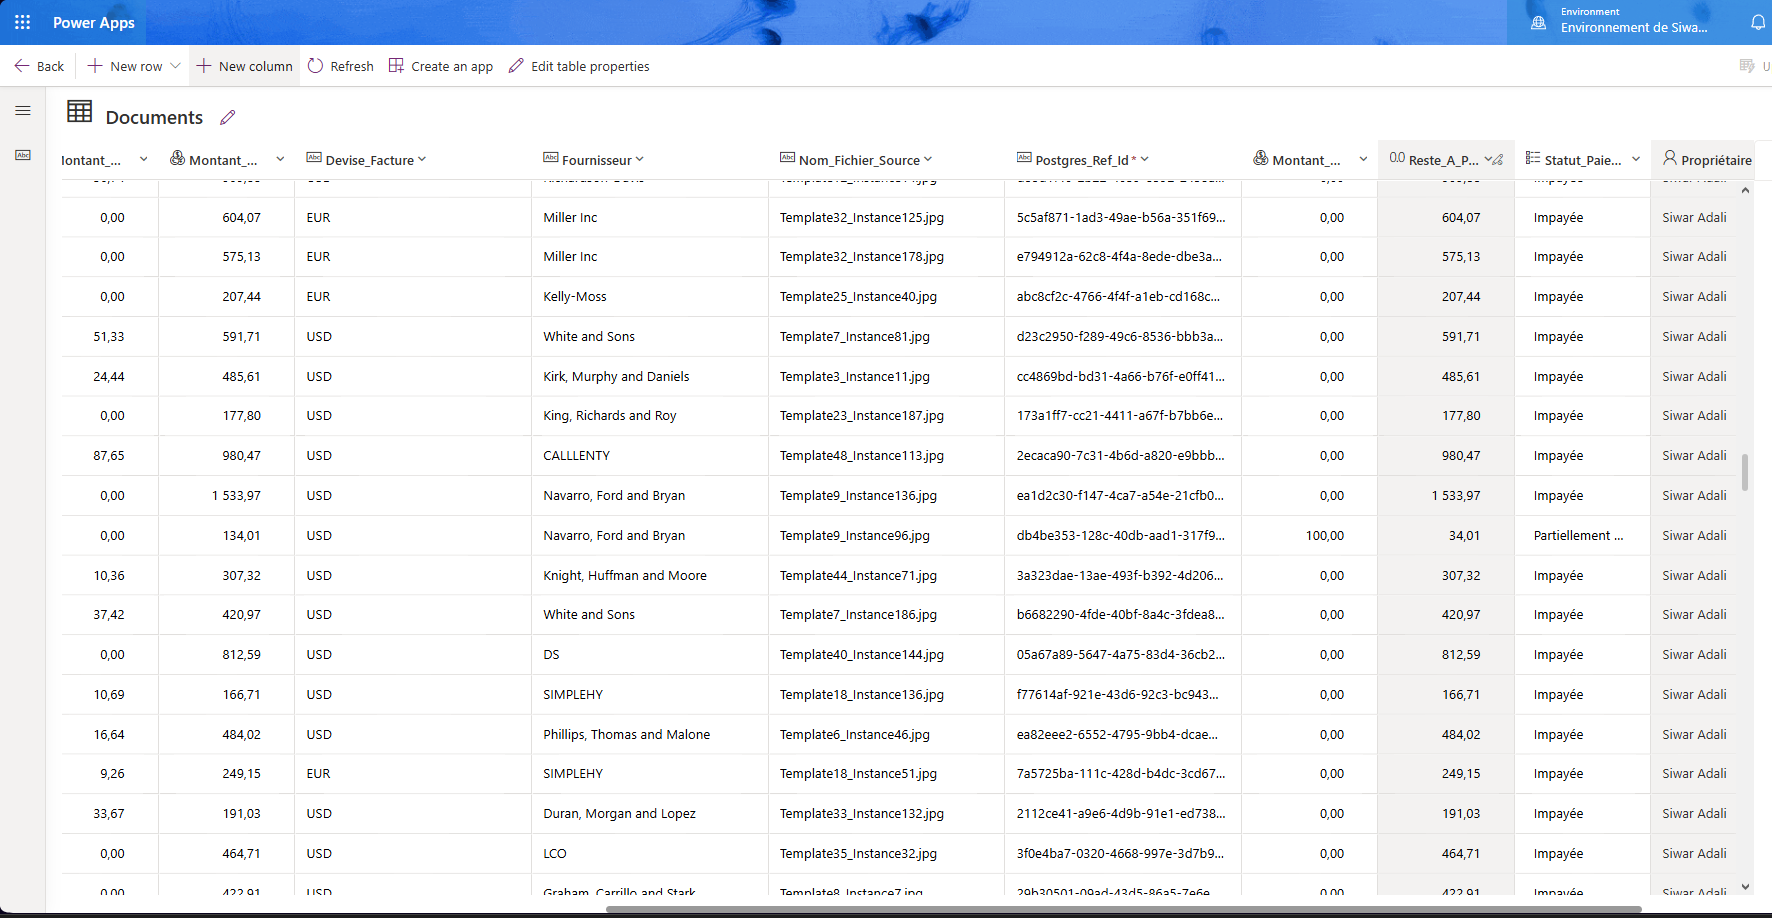
\includegraphics[width=0.85\textwidth]{images/table_Documents_Dataverse.png}
\caption[Table Documents Dataverse]{Vue de la table Documents dans Dataverse apres synchronisation.}
\label{fig:table-documents-dataverse}
\end{figure}

\section{Formulaire Power Apps}

Le formulaire Power Apps, appele \textit{Outil de facturation}, affiche les informations extraites. Les champs issus de l'extraction sont verrouilles en lecture seule afin d'eviter une modification accidentelle des donnees sources. Le champ \texttt{Montant\_Paye}, lui, reste editable pour permettre a l'utilisateur de saisir l'avancement du paiement.

\begin{figure}[H]
\center
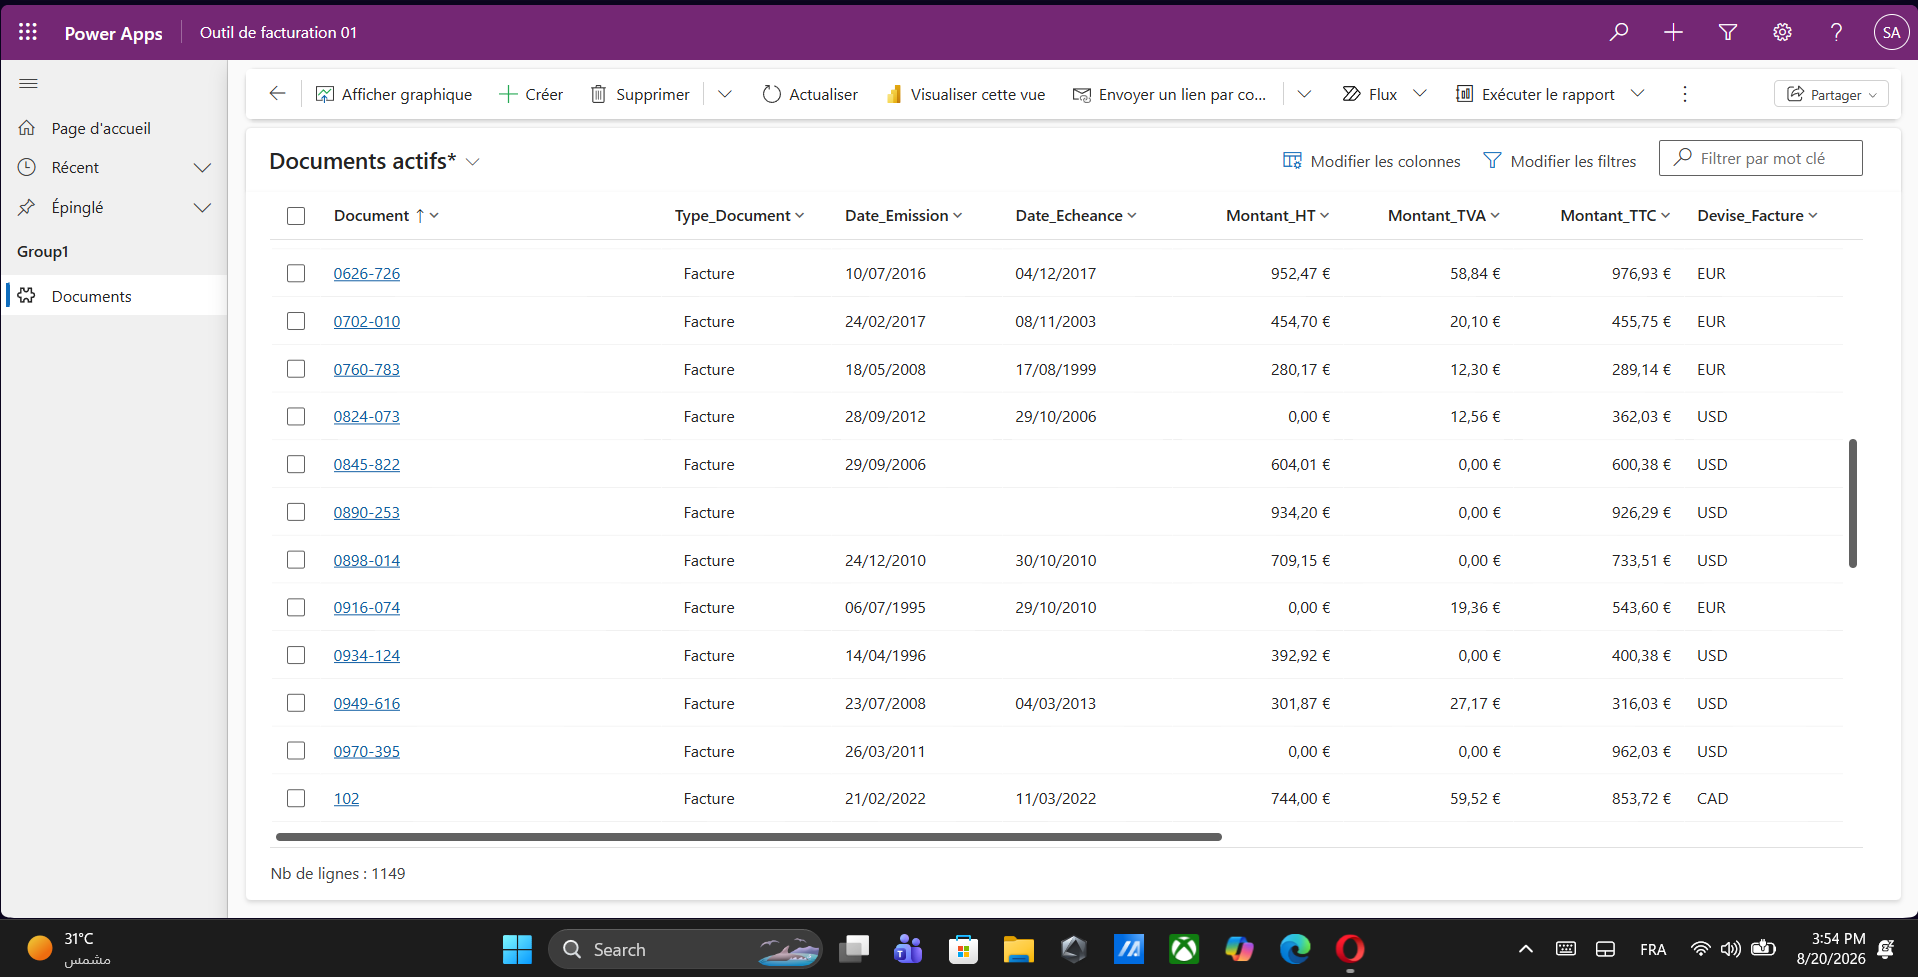
\includegraphics[width=0.9\textwidth]{images/outil_de_facturation.png}
\caption[Outil de facturation Power Apps]{Formulaire Power Apps utilise pour consulter les donnees extraites et saisir le montant paye.}
\label{fig:outil-facturation}
\end{figure}

\begin{figure}[H]
\center
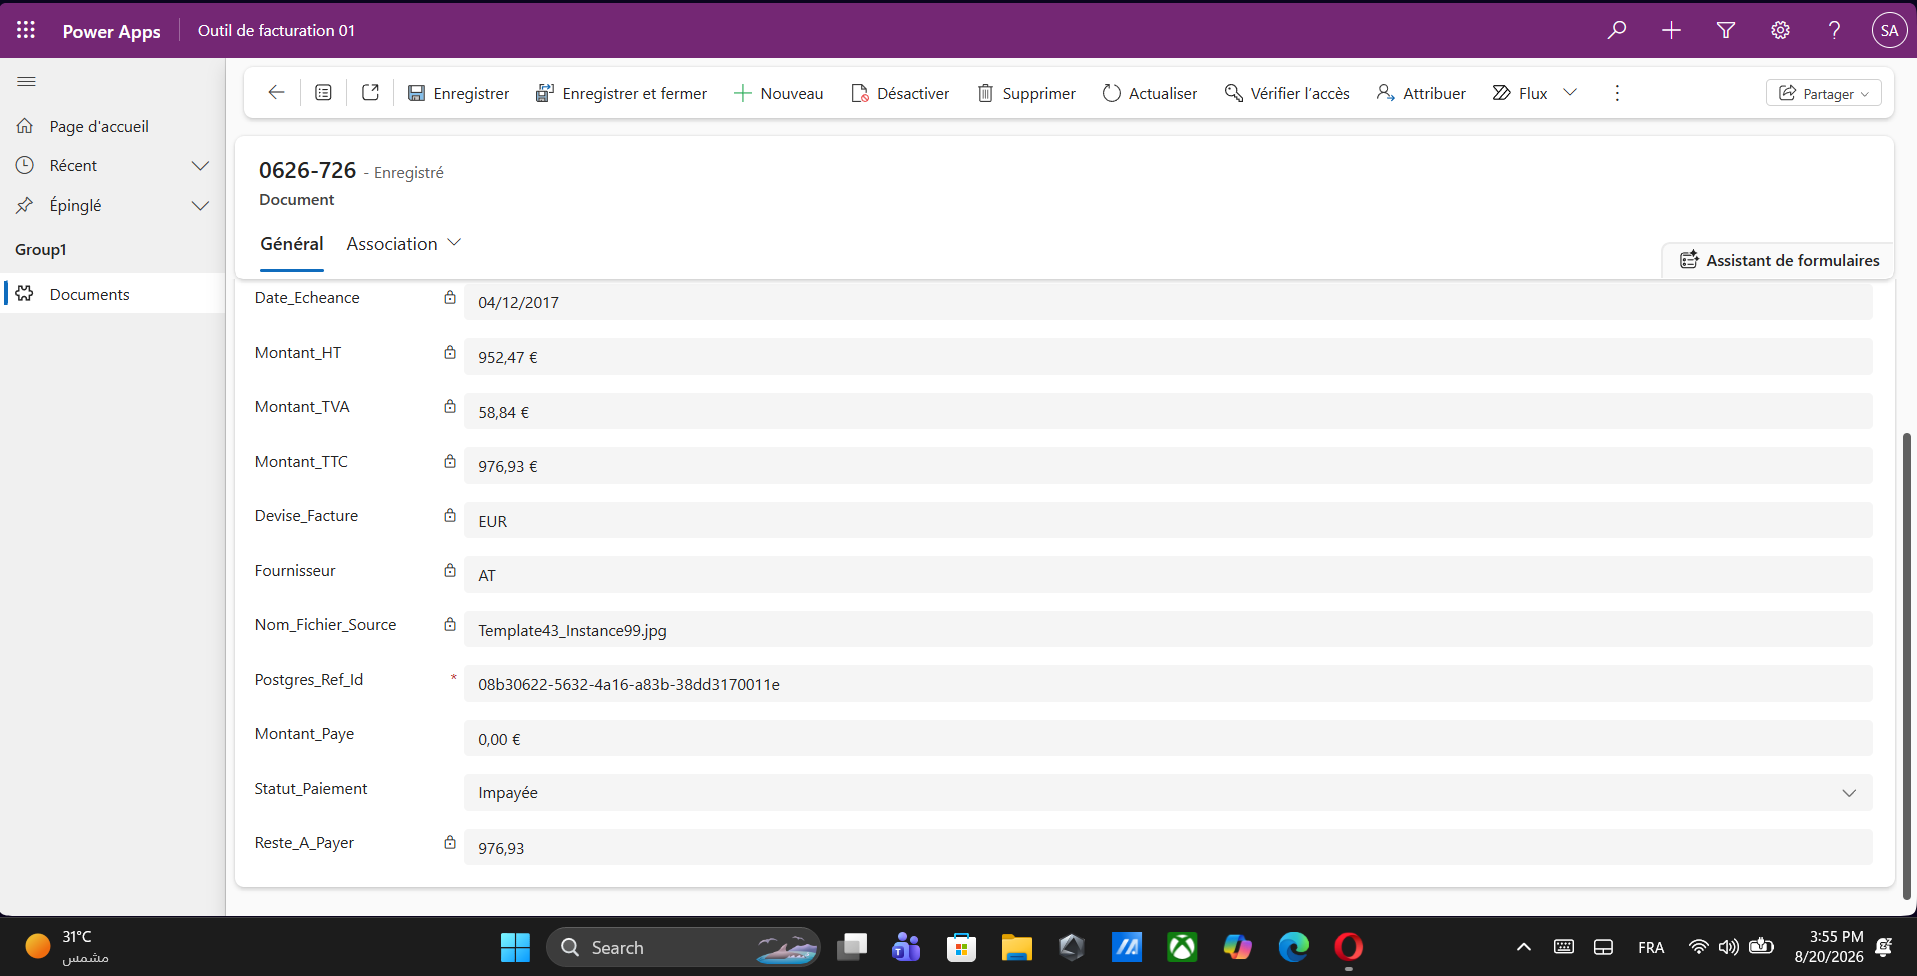
\includegraphics[width=0.8\textwidth]{images/exemple_facture.png}
\caption[Exemple de facture affichee]{Exemple de facture utilisee pour valider l'affichage des champs dans l'outil de facturation.}
\label{fig:exemple-facture}
\end{figure}

\section{Synchronisation du paiement}

Le deuxieme flux Power Automate synchronise le montant paye saisi dans Power Apps vers Postgres. La colonne \texttt{reste\_a\_payer} est calculee automatiquement comme colonne generee SQL, ce qui evite de dupliquer une logique de calcul dans plusieurs outils.

\begin{figure}[H]
\center
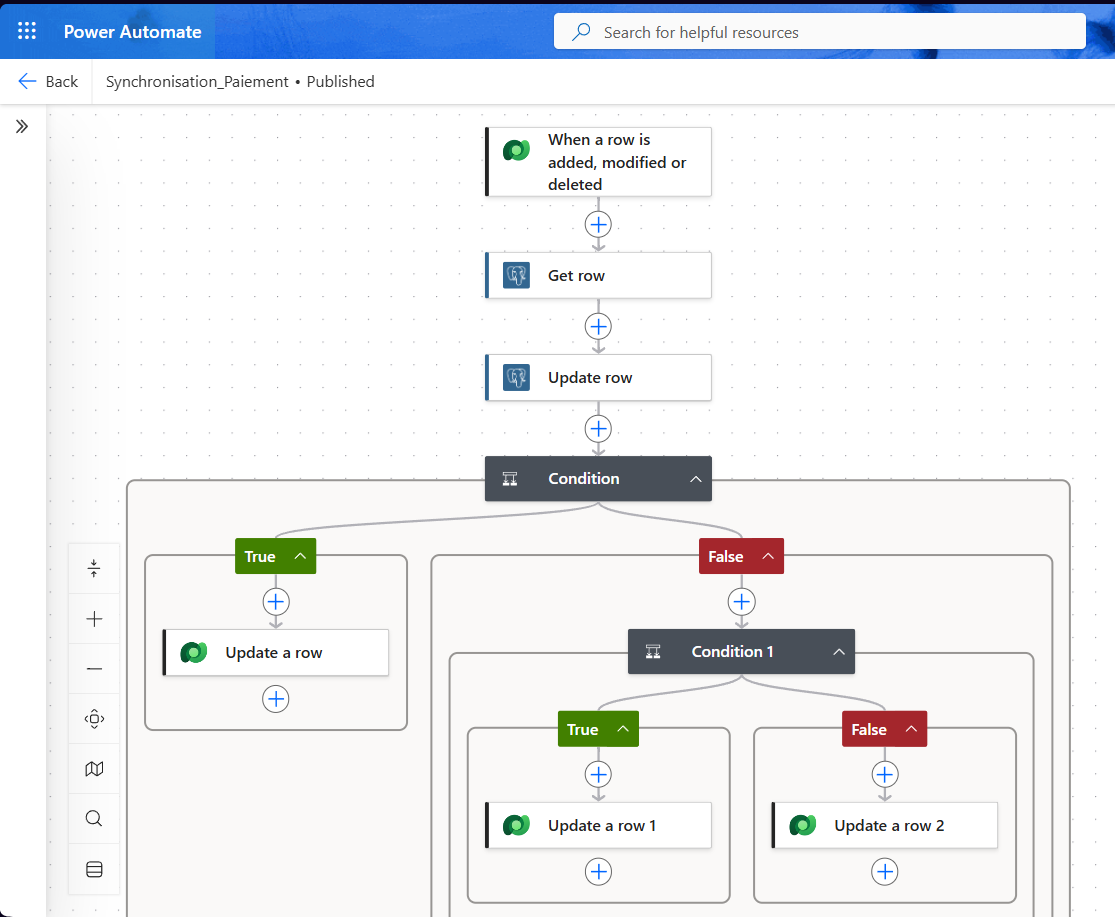
\includegraphics[width=0.9\textwidth]{images/flow2.png}
\caption[Flux de retour paiement]{Flux Power Automate qui renvoie le montant paye depuis Dataverse vers Postgres.}
\label{fig:flow2}
\end{figure}

\begin{figure}[H]
\center
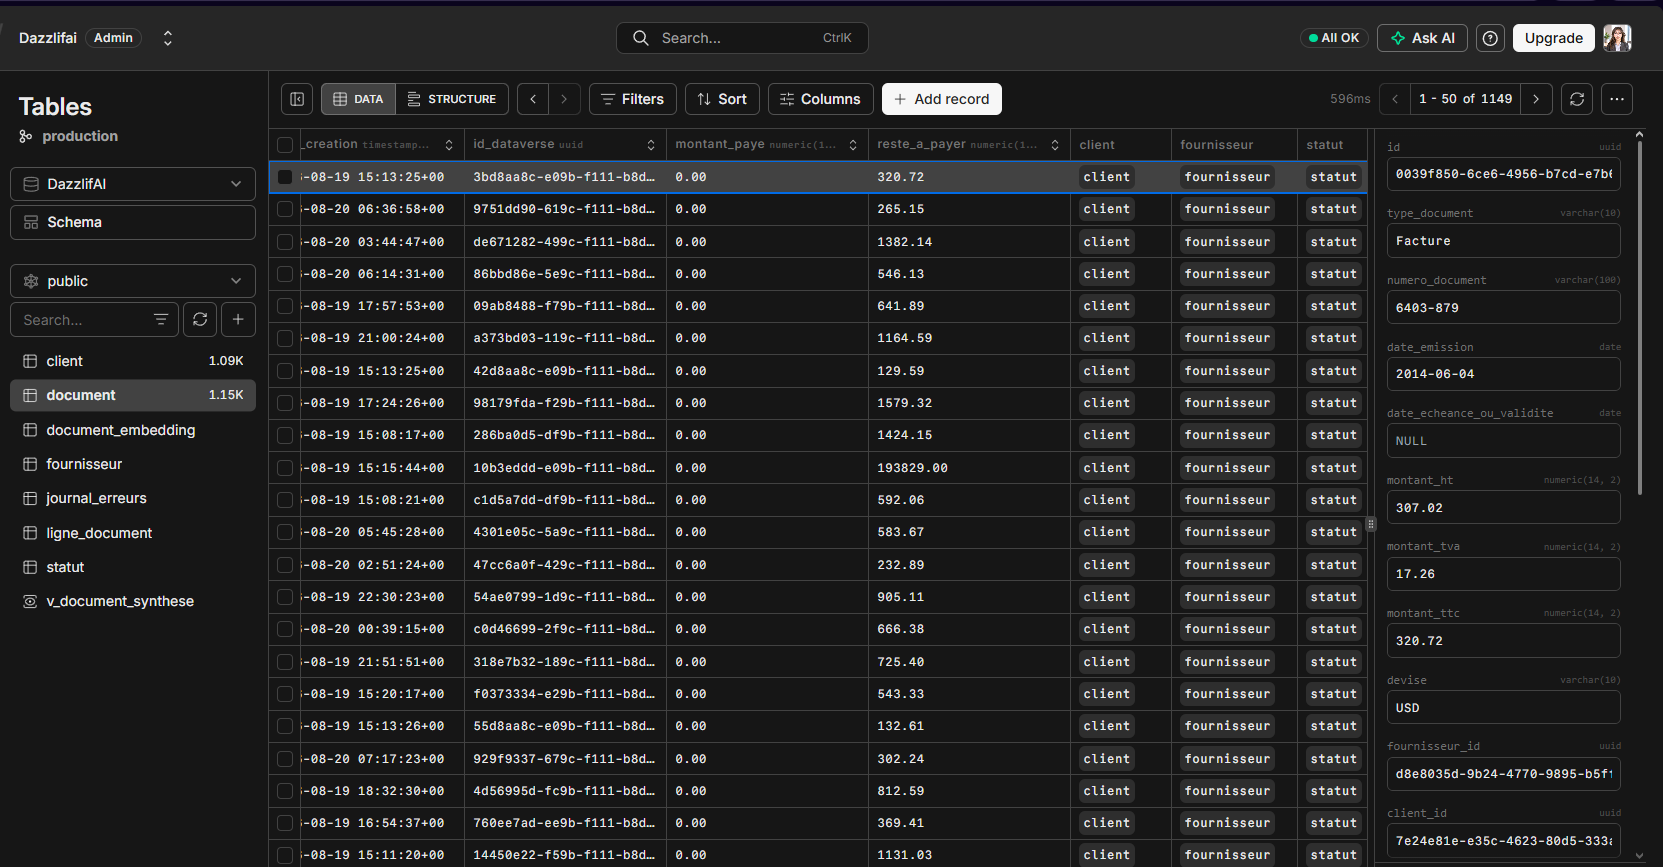
\includegraphics[width=0.85\textwidth]{images/ajout_montant_paye_et_reste_a_payer.png}
\caption[Colonnes de paiement Postgres]{Ajout du montant paye et du reste a payer dans le schema Postgres.}
\label{fig:montant-reste}
\end{figure}

\section{Bugs resolus pendant l'integration}

Plusieurs problemes concrets ont ete rencontres. Une erreur \texttt{ODataUnrecognizedPathException} est apparue a cause d'un champ \texttt{Owner} mal mappe dans Dataverse. La correction a consiste a revoir le nom logique du champ et la maniere dont Power Automate construisait la requete.

Une deuxieme difficulte concernait une confusion entre un identifiant UUID et une URL OData. Le flux transmettait une valeur au mauvais format, ce qui empechait Dataverse de resoudre correctement la ligne cible. La solution a ete de separer clairement l'identifiant brut, utilise cote Postgres, et la reference OData attendue par Dataverse.

Enfin, une incoherence de precision monetaire a ete observee. Les colonnes \texttt{Currency} de Dataverse arrondissaient certaines valeurs a 0 decimale, alors que Postgres stockait les montants en \texttt{NUMERIC(14,2)}. Ce point a ete corrige en ajustant les types et en validant la precision des valeurs synchronisees.
